%!TEX root = main.tex
\resetcounters
\chapter{Concepts of Polytopes}\label{ch:concepts:sec:polytopes}
%
%
%
%
In the previous section we outlined the basic concepts of the robust model predictive control problems we discuss in this work.
%
For general systems and constraint sets it is not possible to efficiently solve the problem~\eqref{ch:concepts:general:rmpc:problem:formulation}, or to explicitly characterise the stage-constraints involved, i.e. the maximal robust positive invariant set~$\X^\infty_{\max}$ and its target tube~$\{\mathcal C_N(\X^\infty_{\max}),\dots,\X^\infty_{\max}\}$.
%
Later we will see that it is possible to formulate~\eqref{ch:concepts:general:rmpc:problem:formulation} for polytopic sets and linear dynamics.
%
To provide an insight into the analysis of such polytopic constraint sets and the necessary computation we present an overview of the required concepts of polytopes.
%
The majority of the concepts summarised here can be found in~\cite{Ziegler:1995,Gruenbaum:1967,Hadwiger:1957}.
%
%
%
%
\section{Descriptions of a Polytope and its Structure}\label{ch:concepts:sec:polytopes:descriptions}
%
%
\mysplit Firstly we characterise the representations of convex polyhedra:
%
\begin{defi}
For the finite point sets~$\{v_i\}_{i\leq M_v}\subset\RR^d$ and $\{r_i\}_{i\leq M_r}\subset\RR^d$ the sets~$\conv\{v_i\}$ and~$\text{cone}\{r_i\}$ given by
%
\begin{equation}\begin{aligned}
	\conv\{v_i\} &= \left\{x\in\RR^d:\exists\lambda_i\geq0\wedge\sum_{i=1}^{M_v}\lambda_i=1\wedge x=\sum_{i=1}^{M_v}\lambda_iv_i\right\}\\
	\text{cone}\{r_i\} &= \left\{x\in\RR^d:\exists \eta_i\geq0\wedge x=\sum_{i=1}^{M_r}\eta_i r_i\right\}
\end{aligned}\end{equation}
%
are called the \emph{convex hull} of $\{v_i\}$ and the \emph{conical hull} of $\{r_i\}$ respectively.
%
The Minkowski sum of the convex hull~$\conv\{v_i\}$ and~$\text{cone}\{r_i\}$
%
\begin{equation}\begin{aligned}
	\X &= \conv\{v_i\}\oplus\text{cone}\{r_i\}\\
	&=\left\{x\in\RR^d:\exists\lambda_i\geq0\wedge\eta_i\geq0\wedge\sum_{i=1}^{M_v}\lambda_i=1\wedge x=\sum_{i=1}^{M_v}\lambda_i v_i+\sum_{i=1}^{M_r}\eta_i r_i\right\}
\end{aligned}\end{equation}
%
is called a $V$-polyhedron.
%
%
For the points~$\{a_i\}_{i\leq M_H}\subset(\RR^d)^\ast$ and~$\{b_i\}_{i\leq M_H}\subset\RR$ the set~$\Y$ given by the intersection of the half-spaces~$H_i = \{x\in\RR^d:a_i x\leq b_i\}$, i.e.
%
\begin{equation}
	\Y=\{x\in\RR^d: a_i x\leq b_i\;\forall i\leq M_H\}
\end{equation}
%
is called a $H$-polyhedron.
%
A polyhedron is called is called a \emph{polytope} if it is bounded.
\end{defi}
%
\noindent We have the statement (see e.g.~\cite{Ziegler:1995}):
%
\begin{thm}
A set~$\X\subseteq\RR^d$ is the Minkowski sum of a convex hull of a finite point set~$\{v_i\}_{i\leq M_v}$ and the conical hull of a finite point set~$\{r_i\}_{i\leq M_r}$, i.e.~$\X=\conv\{v_i\}\oplus\text{cone}\{r_i\}$ iff it is the  intersection of a finite number of closed half-spaces~$\X=\cap H_i$ for some~$\{a_i\}_{i\leq M_H}\subset(\RR^d)^\ast$ and~$\{b_i\}_{i\leq M_H}\subset\RR$.
\end{thm}
%
\noindent This means in particular that there is no reason to distinguish between $V$- and $H$-polyhedra and we therefore omit the $V$- and $H$- in the sequel, we do however refer to a polyhedron for which the \emph{vertices}~$\{v_i\}$ and the \emph{rays}~$\{r_i\}$ are known to be in \emph{vertex representation}.
%
Analogously we say a polyhedron is in \emph{half-space representation} if the \emph{hyperplanes} supporting the half-space~$H_i=\{x:a_i x\leq b_i\}$ are known.
%
\begin{defi}
For the polyhedron~$\X$ a \emph{face} is any non-empty set that can be written as~$F = \X\cap\{x\in\RR^d: c_i x = \hat c_i, i\leq M_F\}$ with $\X\subseteq\{x\in\RR^d: c_ix\leq \hat c_i, i\leq M_F\}$.
%
The \emph{dimension of the face}~$\text{dim}(F)$ is given by the dimension of the hyperplane(s) supporting the face, i.e.~$\text{dim}(F)=\text{dim}(\{x\in\RR^d: c_i x = \hat c_i, i\leq M_F\})$.
%
For a $d$-dimensional polytope a $(d-1)$-dimensional face is called \emph{a facet}, a two-dimensional face \emph{an edge} and a one-dimensional face~\emph{a vertex}.
\end{defi}
%
\noindent Computationally the process of obtaining a vertex representation from a polyhedron in half-space representation is called~\emph{vertex enumeration} and obtaining the half-space representation from a polyhedron in vertex representation is analogously called~\emph{facet enumeration}, as we will see shortly these problems are dual to one another and there are three different algorithms to compute them:
%
The reverse search vertex enumeration~\cite{Avis:2000} implemented in the LRS library, the double description method~\cite{Fukuda:1996} implemented in the CDD library and the primal-dual method~\cite{Bremner:1998} implemented in the PD library.
%
For all our purposes it is not relevant how we switch between the two representations, however all enumeration problems in this work were solved using the LRS library\footnote{For the ease of use the author implemented an interface to Matlab which is publicly available at~\href{http://worc4021.github.io}{http://worc4021.github.io}}.
%
\begin{defi}
The polyhedron~$\X=\cap H_i\subseteq\RR^d$ is called~$\emph{simple}$ if there exists no point~$x\in\X$ which lies on more than~$d$-supporting hyperplanes, it is called \emph{simplicial} if it is the convex hull of exactly~$d+1$ points.
\end{defi}

%
\noindent\mysplit From here on we only present statements for polytopes, equivalent statements can be made for unbounded polyhedra by using slight extensions.
%
\begin{defi}
Let~$\X\subset\RR^d$ be a polytope then its \emph{homogenisation}~$\text{homog}(\X)$ is given by
%
\begin{equation}
	\text{homog}(\X) = \{(tx,t):x\in\X\wedge t>0\}
\end{equation}
\end{defi}
%
\begin{defi}
Let~$\X\subseteq\RR^d$ then the \emph{polar set}~$\X^\tr\subseteq(\RR^d)^\ast$ is defined by
%
\begin{equation}
	\X^\tr := \{c\in(\RR^d)^\ast:cx\leq1\;\forall x\in\X\}.
\end{equation}
\end{defi}
%
\noindent The polar polytope is of particular importance for polytopes which contain the origin in their interior.
%
\begin{thm}
Let~$\X\subset\RR^d=\{x:a_ix\leq 1\}$ be a polytope with the origin in its interior~$0\in\X$, then~$\X^\tr=\conv\{a_i^T\}=\{a:aV\leq\bfa{1}\}$ with $V=(v_1,\dots,v_{M_V})$.
\end{thm}
%
\noindent This means that enumerating the vertices of a polytope is equivalent to determining the half-space description of its polar and vice versa since~$0\in\X$ implies $\X^{\tr\tr}=\X$.
%
\\[1em]
%
An important operation on polytopes (and polyhedra in general) is the projection onto a lower dimension.
%
\begin{defi}
Let~$\X\subseteq\RR^d$ be a polytope and let $1\leq n<d$ then $\pi_n(\X)$ denotes the projection of $\X$ onto~$\RR^n$, i.e.
%
\begin{equation}
	\pi_n(\X) = \{x\in\RR^n:\exists \hat x\in\RR^{d-n} (x,\hat x)\in\X\}.
\end{equation}
\end{defi}
%
\noindent Again there are various methods of computing the projection of a polytope onto a lower dimensional one: 
%
The most trivial one is to \emph{drop} the last $d-n$ elements of all vertices and rays and compute their convex/conical hull.
%
Another, even more computationally wasteful, way is to use the Fourier-Motzkin (see e.g.~\cite{Ziegler:1995}) elimination method $n$~times, which introduces a prohibitive number of redundant hyperplanes.
%
Another method which is available for polytope projection is the equality set projection, see~\cite{Jones:2004} which is less computationally exhaustive but does not cope with unbounded directions.
%
\\[1em]
%
\mysplit Apart from their half-space and vertex representation polytopes can be characterised by their \emph{combinatorial structure}. 
%
Recall that faces are the intersection of hyperplanes with the polytope, statements as \emph{two or more distinct hyperplanes have a non-empty intersection} are either true or false, hence a statement about which hyperplanes define which faces allows us to distil the structure of individual faces and therefore of the entire polytope.
%
While the numerical representation of hyperplanes is non-unique, the hyperplane itself is unique, notice that a facet is supported by exactly one hyperplane, an edge by exactly~$d-1$ hyperplanes and so on. 
%
It is therefore sensible to use this imposed structure to classify polytopes.
%
\begin{defi}
Let~$\X,\Y\subset\RR^d$ be polytopes, then they are called \emph{combinatorially equivalent} if there exists a bijection~$\Pi$ between their faces which preserves the inclusion relation, we denote this by~$\X\cong\Y$.
%
That is if~$F_i\subseteq\X$ is a face of $\X$ then $\Pi(F_i)\subseteq\Y$ is a face of~$\Y$ and furthermore if~$F_j\subseteq\X$ produces a non-empty intersection~$F_i\cap F_j=F_k$ then~$\Pi(F_i)\cap\Pi(F_j)=\Pi(F_k)$.
\end{defi}
%
\noindent There are some cases of trivial equivalences, e.g. every simplicial polytope is combinatorially equivalent to the standard simplex~$\{x\in\RR^d:x_i\geq0\wedge\sum_{i=1}^d x_i=1\}$, however usually it is not trivial to recognise equivalence of combinatorial structure of polytopes.
%
To facilitate the study of the combinatorial structure of polytopes there are several ways to isolate their combinatorial properties.
%
Here we present two:
%
\begin{defi}
The \emph{face lattice}~$L(\X)$ is the partially ordered set of the faces of the polytope~$\X$ for which the order is imposed by the inclusion.
\end{defi}
%
\noindent The study of partially ordered sets is a field in itself, however the concept we need here is quite simple so we illustrate it by example.
%
\begin{example}{The face lattice of a three dimensional cube}\label{example:face:lattice}
Consider the three dimensional cube
%
\[
\X = \left\{x\in\RR^3:\begin{aligned}x_1\leq1\wedge x_2\leq1\wedge x_3\leq 1\wedge\\
-x_1\leq1\wedge -x_2\leq1\wedge -x_3\leq 1\end{aligned}\right\}
\]
%
and its two dimensional faces (facets)~$F_i=\{x:x_i=1\}$ for $i=1,2,3$ and $F_i=\{x:-x_{i-3}=1\}$ for $i=4,5,6$.
%
For this, and in fact for all other three dimensional cubes, we illustrate the face lattice~$L(\X)$ in Figure~\ref{fig:example:face:lattice}.
%
It is now easy to see that the face lattice encloses all combinatorial information there is in a polytope.
%
\begin{figure}\centering
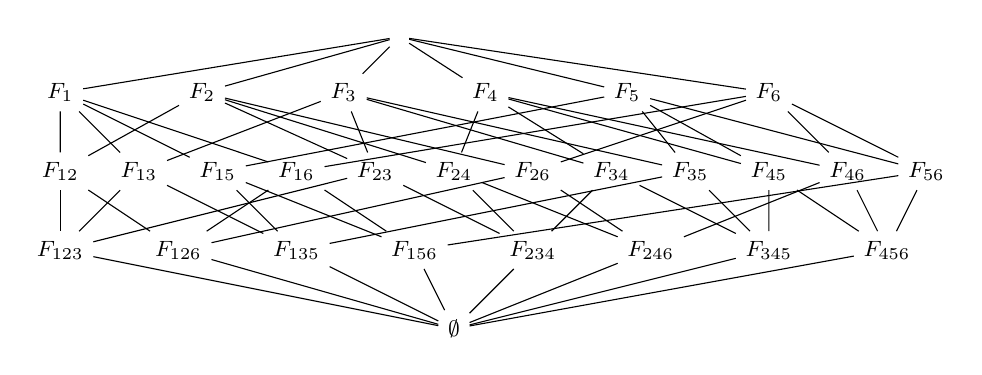
\begin{tikzpicture}
\node (toplevel) {{\footnotesize{$\X$}}};
\node (F3) [below left of=toplevel] {\footnotesize{{$F_3$}}};
\node (F4) [right of=F3,xshift=.8cm] {\footnotesize{{$F_4$}}};
\node (F2) [left of=F3,xshift=-.8cm] {\footnotesize{{$F_2$}}};
\node (F1) [left of=F2,xshift=-.8cm] {\footnotesize{{$F_1$}}};
\node (F5) [right of=F4,xshift=.8cm] {\footnotesize{{$F_5$}}};
\node (F6) [right of=F5,xshift=.8cm] {\footnotesize{{$F_6$}}};
\node (F12) [below of=F1] {\footnotesize{{$F_{12}$}}};
\node (F13) [right of=F12] {\footnotesize{{$F_{13}$}}};
\node (F15) [right of=F13] {\footnotesize{{$F_{15}$}}};
\node (F16) [right of=F15] {\footnotesize{{$F_{16}$}}};
\node (F23) [right of=F16] {\footnotesize{{$F_{23}$}}};
\node (F24) [right of=F23] {\footnotesize{{$F_{24}$}}};
\node (F26) [right of=F24] {\footnotesize{{$F_{26}$}}};
\node (F34) [right of=F26] {\footnotesize{{$F_{34}$}}};
\node (F35) [right of=F34] {\footnotesize{{$F_{35}$}}};
\node (F45) [right of=F35] {\footnotesize{{$F_{45}$}}};
\node (F46) [right of=F45] {\footnotesize{{$F_{46}$}}};
\node (F56) [right of=F46] {\footnotesize{{$F_{56}$}}};
\node (F123) [below of=F12] {\footnotesize{$F_{123}$}};
\node (F126) [right of=F123,xshift=.5cm] {\footnotesize{$F_{126}$}};
\node (F135) [right of=F126,xshift=.5cm] {\footnotesize{$F_{135}$}};
\node (F156) [right of=F135,xshift=.5cm] {\footnotesize{$F_{156}$}};
\node (F234) [right of=F156,xshift=.5cm] {\footnotesize{$F_{234}$}};
\node (F246) [right of=F234,xshift=.5cm] {\footnotesize{$F_{246}$}};
\node (F345) [right of=F246,xshift=.5cm] {\footnotesize{$F_{345}$}};
\node (F456) [right of=F345,xshift=.5cm] {\footnotesize{$F_{456}$}};
\node (empty) [below of=F123,xshift=5cm] {\footnotesize{$\emptyset$}};
\draw (toplevel) -- (F1);
\draw (toplevel) -- (F2);
\draw (toplevel) -- (F3);
\draw (toplevel) -- (F4);
\draw (toplevel) -- (F5);
\draw (toplevel) -- (F6);
\draw (F1) -- (F12) -- (F2);
\draw (F1) -- (F13) -- (F3);
\draw (F1) -- (F15) -- (F5);
\draw (F1) -- (F16) -- (F6);
\draw (F2) -- (F23) -- (F3);
\draw (F2) -- (F24) -- (F4);
\draw (F2) -- (F26) -- (F6);
\draw (F3) -- (F34) -- (F4);
\draw (F3) -- (F35) -- (F5);
\draw (F4) -- (F45) -- (F5);
\draw (F4) -- (F46) -- (F6);
\draw (F5) -- (F56) -- (F6);
\draw (F12) -- (F123);
\draw (F13) -- (F123);
\draw (F23) -- (F123);
\draw (F12) -- (F126);
\draw (F16) -- (F126);
\draw (F26) -- (F126);
\draw (F13) -- (F135);
\draw (F15) -- (F135);
\draw (F35) -- (F135);
\draw (F15) -- (F156);
\draw (F16) -- (F156);
\draw (F56) -- (F156);
\draw (F23) -- (F234);
\draw (F24) -- (F234);
\draw (F34) -- (F234);
\draw (F24) -- (F246);
\draw (F26) -- (F246);
\draw (F46) -- (F246);
\draw (F34) -- (F345);
\draw (F35) -- (F345);
\draw (F45) -- (F345);
\draw (F45) -- (F456);
\draw (F46) -- (F456);
\draw (F56) -- (F456);
\draw (F123) -- (empty);
\draw (F126) -- (empty);
\draw (F135) -- (empty);
\draw (F156) -- (empty);
\draw (F234) -- (empty);
\draw (F246) -- (empty);
\draw (F345) -- (empty);
\draw (F456) -- (empty);
\end{tikzpicture}
\\[1em]
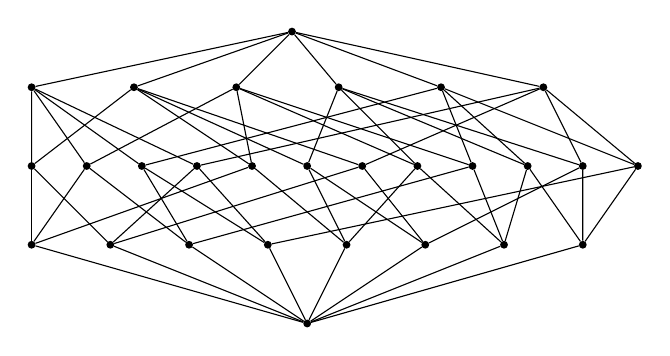
\begin{tikzpicture}
\node (toplevel) [circle,fill,scale=.3] {};
\node (F3) [below left of=toplevel,circle,fill,scale=.3] {};
\node (F4) [right of=F3,xshift=.3cm,circle,fill,scale=.3] {};
\node (F2) [left of=F3,xshift=-.3cm,circle,fill,scale=.3] {};
\node (F1) [left of=F2,xshift=-.3cm,circle,fill,scale=.3] {};
\node (F5) [right of=F4,xshift=.3cm,circle,fill,scale=.3] {};
\node (F6) [right of=F5,xshift=.3cm,circle,fill,scale=.3] {};
\node (F12) [below of=F1,circle,fill,scale=.3] {};
\node (F13) [right of=F12,xshift=-.3cm,circle,fill,scale=.3] {};
\node (F15) [right of=F13,xshift=-.3cm,circle,fill,scale=.3] {};
\node (F16) [right of=F15,xshift=-.3cm,circle,fill,scale=.3] {};
\node (F23) [right of=F16,xshift=-.3cm,circle,fill,scale=.3] {};
\node (F24) [right of=F23,xshift=-.3cm,circle,fill,scale=.3] {};
\node (F26) [right of=F24,xshift=-.3cm,circle,fill,scale=.3] {};
\node (F34) [right of=F26,xshift=-.3cm,circle,fill,scale=.3] {};
\node (F35) [right of=F34,xshift=-.3cm,circle,fill,scale=.3] {};
\node (F45) [right of=F35,xshift=-.3cm,circle,fill,scale=.3] {};
\node (F46) [right of=F45,xshift=-.3cm,circle,fill,scale=.3] {};
\node (F56) [right of=F46,xshift=-.3cm,circle,fill,scale=.3] {};
\node (F123) [below of=F12,circle,fill,scale=.3] {};
\node (F126) [right of=F123,circle,fill,scale=.3] {};
\node (F135) [right of=F126,circle,fill,scale=.3] {};
\node (F156) [right of=F135,circle,fill,scale=.3] {};
\node (F234) [right of=F156,circle,fill,scale=.3] {};
\node (F246) [right of=F234,circle,fill,scale=.3] {};
\node (F345) [right of=F246,circle,fill,scale=.3] {};
\node (F456) [right of=F345,circle,fill,scale=.3] {};
\node (empty) [below of=F123,xshift=3.5cm,circle,fill,scale=.3] {};
\draw (toplevel) -- (F1);
\draw (toplevel) -- (F2);
\draw (toplevel) -- (F3);
\draw (toplevel) -- (F4);
\draw (toplevel) -- (F5);
\draw (toplevel) -- (F6);
\draw (F1) -- (F12) -- (F2);
\draw (F1) -- (F13) -- (F3);
\draw (F1) -- (F15) -- (F5);
\draw (F1) -- (F16) -- (F6);
\draw (F2) -- (F23) -- (F3);
\draw (F2) -- (F24) -- (F4);
\draw (F2) -- (F26) -- (F6);
\draw (F3) -- (F34) -- (F4);
\draw (F3) -- (F35) -- (F5);
\draw (F4) -- (F45) -- (F5);
\draw (F4) -- (F46) -- (F6);
\draw (F5) -- (F56) -- (F6);
\draw (F12) -- (F123);
\draw (F13) -- (F123);
\draw (F23) -- (F123);
\draw (F12) -- (F126);
\draw (F16) -- (F126);
\draw (F26) -- (F126);
\draw (F13) -- (F135);
\draw (F15) -- (F135);
\draw (F35) -- (F135);
\draw (F15) -- (F156);
\draw (F16) -- (F156);
\draw (F56) -- (F156);
\draw (F23) -- (F234);
\draw (F24) -- (F234);
\draw (F34) -- (F234);
\draw (F24) -- (F246);
\draw (F26) -- (F246);
\draw (F46) -- (F246);
\draw (F34) -- (F345);
\draw (F35) -- (F345);
\draw (F45) -- (F345);
\draw (F45) -- (F456);
\draw (F46) -- (F456);
\draw (F56) -- (F456);
\draw (F123) -- (empty);
\draw (F126) -- (empty);
\draw (F135) -- (empty);
\draw (F156) -- (empty);
\draw (F234) -- (empty);
\draw (F246) -- (empty);
\draw (F345) -- (empty);
\draw (F456) -- (empty);
\end{tikzpicture}
\caption[Face lattice of a cube]{The face lattice~$L(\X)$ of the three dimensional cube~$\X$ in Example~\ref{example:face:lattice}.
Here we abbreviate~$F_{ij}=F_i\cap F_j$ and $F_{ijk}=F_i\cap F_j\cap F_k$.
Usually the names we give the faces are irrelevant so that the face lattice is illustrated as in the lower figure.}
\label{fig:example:face:lattice}
\end{figure}
%
\end{example}
%
It is worth pointing out that the combinatorial structure does not hold all the structural information there is about a polytope, for example for polytopes that contain the origin in their interior~$0\in\X$ the bipolar polytope~$\X^{\tr\tr}=\X$ is the polytope itself.
%
In particular the face lattice of the polar polytope is then the partially ordered set with inverted order, i.e. visually the lattice is flipped upside down.
%
However, there exist translations~$p\in\RR^d$ such that the origin is no longer in the interior~$0\not\in\X\oplus\{p\}$ and therefore the polar of the polytope is empty (hence the bipolar is empty as well), yet the face lattice does not change.
%
And yet, knowing the combinatorial structure of a polytope does enable us to perform a variety of additional computations.
%
In the sequel of this work we will not explicitly use the face lattice to study the combinatorial structure of polytopes, however they illustrate the entire combinatorial structure of a polytope in a simple way and are hence the preferred representation to think about combinatorial structure of a polytope.
%
\\[1em]
%
Instead of using the entire face lattice we use another description which illustrates the combinatorial structure only on the lowest two dimensions, i.e. only vertices and edges are used to encode the entire combinatorial structure of a polytope.
%
\begin{defi}
Let~$\X\subset\RR^d$ be a polytope then~$\mathcal G(\X)=(\mathcal V,\mathcal E)$ denotes its \emph{induced graph}.
%
The vertex set~$\mathcal V$ is given by the vertices of the polytope, the edge set~$\mathcal E$ is given by its edge set.
\end{defi}
%
\noindent We illustrate the induced graph for the cube in Example~\ref{example:face:lattice} in Figure~\ref{fig:example:induced:graph}.
%
The induced graph of a polytope is of major interest when studying the simplex algorithm for linear programming since it 'walks down a path along vertices of the induced graph' until reaching the optimum, see e.g.~\cite{Ziegler:1995}.
%
\begin{figure}\centering
\tdplotsetmaincoords{65}{40}
\begin{tikzpicture}[tdplot_main_coords]
\node at ( -1.0000,  -1.0000, -1.0000) [circle,fill,scale=.3] {};
\node at (  1.0000,  -1.0000, -1.0000) [circle,fill,scale=.3] {};
\node at ( -1.0000,   1.0000, -1.0000) [circle,fill,scale=.3] {};
\node at (  1.0000,   1.0000, -1.0000) [circle,fill,scale=.3] {};
\node at ( -1.0000,  -1.0000,  1.0000) [circle,fill,scale=.3] {};
\node at (  1.0000,  -1.0000,  1.0000) [circle,fill,scale=.3] {};
\node at ( -1.0000,   1.0000,  1.0000) [circle,fill,scale=.3] {};{}
\node at (  1.0000,   1.0000,  1.0000) [circle,fill,scale=.3] {};

\draw (  1.0000,  -1.0000,  -1.0000) -- (  1.0000,   1.0000,  -1.0000) -- (  1.0000,   1.0000,   1.0000) -- (  1.0000,  -1.0000,   1.0000) -- (  1.0000,  -1.0000,  -1.0000) -- cycle;

\draw ( -1.0000,   1.0000,  -1.0000) -- ( -1.0000,   1.0000,   1.0000) -- (  1.0000,   1.0000,   1.0000) -- (  1.0000,   1.0000,  -1.0000) -- ( -1.0000,   1.0000,  -1.0000) -- cycle;

\draw ( -1.0000,  -1.0000,   1.0000) -- (  1.0000,  -1.0000,   1.0000) -- (  1.0000,   1.0000,   1.0000) -- ( -1.0000,   1.0000,   1.0000) -- ( -1.0000,  -1.0000,   1.0000) -- cycle;

\draw ( -1.0000,  -1.0000,  -1.0000) -- ( -1.0000,   1.0000,  -1.0000) -- ( -1.0000,   1.0000,   1.0000) -- ( -1.0000,  -1.0000,   1.0000) -- ( -1.0000,  -1.0000,  -1.0000) -- cycle;

\draw ( -1.0000,  -1.0000,  -1.0000) -- ( -1.0000,   1.0000,  -1.0000) -- (  1.0000,   1.0000,  -1.0000) -- (  1.0000,  -1.0000,  -1.0000) -- ( -1.0000,  -1.0000,  -1.0000) -- cycle;

\draw ( -1.0000,  -1.0000,  -1.0000) -- (  1.0000,  -1.0000,  -1.0000) -- (  1.0000,  -1.0000,   1.0000) -- ( -1.0000,  -1.0000,   1.0000) -- ( -1.0000,  -1.0000,  -1.0000) -- cycle;
\end{tikzpicture}
\caption[Induced graph of a cube]{The induced graph~$\mathcal G(\X)$ of the cube in Example~\ref{example:face:lattice}.}
\label{fig:example:induced:graph}
\end{figure}
%
%
In particular we have that the induced graph of every $d$-dimensional polytope is $d$-connected, i.e. every vertex has at least $d$ edges, see~\cite{Balinski:1961}.
%
The converse is also true, i.e. a $d$-connected graph defines the combinatorial structure of a $d$-dimensional polytope~\cite{Kalai:1988}.
%
And furthermore we have the following connecting statement
%
\begin{thm}
If $\X\subset\RR^d$ is a simple polytope, then its induced graph~$\mathcal G(\X)$ determines the entire combinatorial structure of~$\X$, i.e. if~$\mathcal G(\X)=\mathcal G(\Y)$ then $L(\X)=L(\Y)$.
\end{thm}
%
\noindent This means that although the induced graph only characterises the one- and two-dimensional faces it contains the same amount of information as the face lattice.
%
In the context of the simplex algorithm we have the problem of determining the longest \emph{diameter} of a graph, for a particular graph~$\mathcal G$ the diameter~$\delta(\mathcal G)$ is the smallest number such that any two vertices of~$\mathcal G$ can be connected by a path with no more than $\delta(\mathcal G)$ edges.
%
Usually the graph is not known in general, so we use~$\Delta(d,n)$ to denote the maximal diameter of a graph of a $d$-dimensional polytope with no more than~$n$ facets\footnote{The definition of having no more than~$n$ facets comes again from linear programming where the number of constraints can be~$n$ but due to redundancies the effective number of constraints may be smaller.}.
%
Originally Warren Hirsch proposed an upper bound for~$\Delta(d,n)$ which was later proven wrong in various instances, however the bounds on~$\Delta(d,n)$ are still referred to as the \emph{Hirsch conjecture}~\cite{Ziegler:2012}.
%
\begin{thm}
Let~$\Delta(d,n)$ denote the maximal diameter of a induced graph of a $d$-dimensional polytope with no more than $n$ facets, then the following bounds hold:
%
\begin{equation}
	\begin{aligned}
	\Delta(d,n) &\leq n^{\log_2(2d)}\\
	\Delta(d,n) &\leq \frac{1}{12}2^dn
	\end{aligned}
\end{equation}
\end{thm}
%
\noindent These bounds are presented in~\cite{Ziegler:2012,Ziegler:1995,Kalai:1992,Barnette:1974}.
%
A survey illustrating the difficulty of obtaining a sub-exponential bound can be found in~\cite{Klee:1987}.
%
\\[1em]
%
The statements on the combinatorial structure of a polytope may seem to be irrelevant in the study of robust model predictive control, however, we will see that knowing the combinatorial structure of a polytope enables us to compute objects with polytopes which otherwise would not be possible.
%
One particular statement that makes this possible is the following.
%
\begin{thm}
Let~$\X\subset\RR^d$ be a polytope, then there exist simplices~$S_1,\dots,S_p$ such that $\text{dim}(S_i)=d$, $\text{int}(S_i\cap S_j)=\emptyset$ and $\X=\bigcup_{i=1}^p S_i$.
%
Furthermore, the induced graphs~$\mathcal G(S_i)=(\mathcal V_i,\mathcal E_i)$ decompose the induced graph~$\mathcal G(\X)=(\mathcal V,\mathcal E)$, i.e.~$\bigcup_i \mathcal G(S_i) = \mathcal G(\X)$ and $\abs{\mathcal V_i\cap \mathcal V_j}=d$, $\mathcal E_i\cap\mathcal E_j=\emptyset$.
\end{thm}
%
\noindent For a proof see e.g.~\cite{Hadwiger:1957,Ziegler:1995}.
%
This means that the \emph{simplex decomposition} for one polytope is applicable for all other polytopes which are combinatorially equivalent.
%
One obvious way of applying this is to simplify the computation of the volume of a polytope.
%
While it is non-trivial to compute the volume of a polytope with direct methods (see e.g.~\cite{Lasserre:2001} for a non-decomposing algorithm) computing the volume of a simplex can be done by computing a single determinant~\cite{Hadwiger:1957}.
%
Hence with the simplex decomposition of~$\X$ the problem of computing its volume becomes the problem of adding up determinants, and with the same method we can compute the volume of any transformation~$f(\X)$ as long as~$f(\X)\cong\X$.
%
We will exploit this fact later on.
%
\\[1em]
%
\mysplit In the context of transformations that preserve the combinatorial structure of a polytope we present a particularly simple one, the \emph{projective transformation}.
%
For the polytope~$\X\subset\RR^d$ the homogenisation~$\text{homog}(\X)=\{(xt,t)\in\RR^{d+1}:x\in\X\wedge t>0\}$ is a pointed cone in $\RR^{d+1}$.
%
Introducing the hyperplane~$H = \{(x,t):t=1\}$ the set~$\text{homog}(\X)\cap H$ is an 'embedded version' of~$\X$ in~$\RR^{d+1}$, i.e. the two sets are isomorphic.
%
In particular the combinatorial structure of~$\X$ is identical with that of~$\X^\prime:=\text{homog}(\X)\cap H$, this can be extended to more hyperplanes~$H = \{(x,t)\in\RR^{d+1}:ax+\tilde a t=1\}$ as long as each ray~$(v_i,1)t$ given by the vertex~$v_i$ of~$\X$ is intersected by~$H$.
%
Clearly this condition is satisfied if
%
\begin{equation}
	\begin{pmatrix}
	a &\tilde a
	\end{pmatrix}\begin{pmatrix}
	v_i\\ 1\end{pmatrix}>0
\end{equation}
%
for all vertices~$v_i$ of~$\X=\conv\{v_i\}$.
%
For such hyperplanes~$H$ it can be shown that the combinatorial structure of~$\X$ is preserved, i.e.~$L(\X)=L(\X^\prime)$, see e.g.~\cite{Garner:1981}.
%
Once more, projective transformations and projective geometry are fields of study in their own right and we merely outline their main idea and refer to~\cite{Garner:1981} for a more detailed presentation.
%
Since the key idea is simple enough to be illustrate in a single diagram we show a projective transformation in Figure~\ref{fig:projective:transformation:explained}.
%
\begin{figure}
\centering
\begin{tikzpicture}
\node (a) at (0,0) {
\begin{tikzpicture}
\draw[-latex'] (0,0) -- (1.3,0) node[below]{$x_1$};
\draw[-latex'] (0,0) -- (0,1.3) node[right]{$x_2$};
\draw[thick] (-1/3,-1/3) -- (1,0) -- (0,1) -- cycle;
\fill[blue,opacity=.3] (-1/3,-1/3) -- (1,0) -- (0,1) -- cycle;
\end{tikzpicture}
};
%
%
\node [right = of a] (b) {
\tdplotsetmaincoords{65}{-40}
\begin{tikzpicture}[tdplot_main_coords]
\draw[-latex'] (0,0,0) -- (0,0,3.5) node[right] {$t$};
\draw[-latex'] (0,0,0) -- (0,2.1,0) node[below] {$x_2$};
\draw[-latex'] (0,0,0) -- (3.5,0,0) node[below] {$x_1$};
\draw[thick] (0,0,0) -- (-1,-1,3);
\draw[thick] (0,0,0) -- (2,-1,3);
\draw[thick] (0,0,0) -- (-1,2,3);
\fill[opacity=.3,blue] (-1/3,-1/3,1) -- (2/3,-1/3,1) -- (-1/3,2/3,1) -- cycle;
\draw (-1/3,-1/3,1) -- (2/3,-1/3,1) -- (-1/3,2/3,1) -- cycle;
\fill[opacity=.3,green] (-0.3704, -0.3704, 1.1111) -- (0.6061, -0.3030, 0.9091) -- (-0.8333, 1.6667, 2.5000) -- cycle;
\draw (-0.3704, -0.3704, 1.1111) -- (0.6061, -0.3030, 0.9091) -- (-0.8333, 1.6667, 2.5000) -- cycle;
\end{tikzpicture}
};
\draw[-latex'] (a) --node[above]{{\tiny{$\text{homog}(\X)$}}} (b) {};
%
%
\node [right = of b] (c) {
\begin{tikzpicture}
\draw[-latex'] (0,0) -- (1.3,0) node[below]{$\tilde x_1$};
\draw[-latex'] (0,0) -- (0,1.3) node[right]{$\tilde x_2$};
\draw[thick] (1.7541,    2.3601) -- (0.4025,   -0.2198) -- (-0.0841,    0.6531) -- cycle;
\fill[opacity=.3,green] (1.7541,    2.3601) -- (0.4025,   -0.2198) -- (-0.0841,    0.6531) -- cycle;
\end{tikzpicture}
};
\draw[-latex'] (b) -- node[above,near start]{{\tiny{$\text{homog}(\X)\cap H$}}} (c) {};
%
%
% \node [right = of c] (d) {
% \begin{tikzpicture}e
% \draw[-latex'] (0,0) -- (1.3,0) node[below]{$\tilde x_1$};
% \draw[-latex'] (0,0) -- (0,1.3) node[right]{$\tilde x_2$};
% \draw[thick] (1.7623, 0.2586) -- (-1.0177, -0.6100) -- (-0.7446, 0.3514) -- cycle;
% \fill[opacity=.3,red] (1.7623, 0.2586) -- (-1.0177, -0.6100) -- (-0.7446, 0.3514) -- cycle;
% \end{tikzpicture}
% };
% \draw[-latex'] (c) -- node[above]{{\tiny{$R(\tilde\W\oplus\{-b\})$}}} (d) {};
\end{tikzpicture}
\caption[The projective transformation of a polytope]{The projective transformation of a \textcolor{blue}{simplicial polytope} step by step.
First the polytope is lifted into its homogenisation then intersected with the desired admissible hyperplane to obtain the \textcolor{green}{projective transformation}, by projecting into the plane~$H$ we obtain a~$d$-dimensional polytope~$\X^\prime\cong\X$, we can apply a rotation and translation to bring it into any desired orientation without changing the combinatorial structure.}
\label{fig:projective:transformation:explained}
\end{figure}
%
%
%
%
\section{Polytopic Complices}\label{ch:concepts:sec:polytopes:complices}
\resetforsection
%
%
%
In this section we present some statements on \emph{polytopic complices} which arise in the solution of multi-parametric quadratic programming problems as we will see later on.
%
\begin{defi}
A \emph{polyhedral complex}~$\mathcal C$ is a finite collection of polyhedra in $\RR^d$ such that: the empty polyhedron is in~$\mathcal C$, if~$\X\in\mathcal C$ then all faces of $\X$ are also in~$\mathcal C$ and for~$\X,\Y\in\mathcal C$ the intersection~$\X\cap\Y=F$ is a face of $\X$ and of~$\Y$ and is also in the compelx~$F\in\mathcal C$.
%
\\[1em]
%
A polyhedral complex is called a \emph{polytopic} or \emph{polytopal complex} if all its elements are bounded.
%
\\[1em]
%
A polytopic complex is called a~\emph{subdivision} if there exists a polyhedron~$\Y\subseteq\RR^d$ such that the underlying set~$\abs{\mathcal C}=\bigcup_{\X_i\in\mathcal C}\X_i = \Y$.
%
A subdivision is called \emph{regular} if there exists a polyhedron~$\mathcal Z\subseteq\RR^{d+1}$ such that all faces $F_i\in\mathcal C$ arise as projections of faces~$H_i$ of $\mathcal Z$ by projection, i.e.~$F_i=\pi_d(H_i)$.
\end{defi}
%
\noindent One particular regular subdivision we will encounter later is the one that arises by projecting the epigraph of a piecewise affine function~$\epi(f)=\{(x,t)\in\RR^{d+1}:f(x)\leq t\}$ for $f(x)=\max_{k}\{c_k x+ b_k\}$.
%
In this case the regular subdivision specifies polyhedra on each of which the function is affine.
%
\begin{example}{The solution of a multi-parametric linear program}\label{example:mplp:induced:complex}
Consider the multi-parametric linear program presented in~\cite{Borrelli:2003}:
%
\begin{equation}
	f(\theta)=\left\{\begin{aligned}
	\min\quad & x_1+x_2+x_3+x_4\\
	\text{s.t.}\quad & -x_1\pm x_5\leq0\\
	& -x_2\pm x_6\leq 0\\
	& -x_3\leq \pm(\theta_1+\theta_2)\\
	& -x_3\mp x_5\leq \pm\theta_2\\
	& -x_4\mp x_5\leq \pm(\theta_1+2\theta_2)\\
	& -x_4\mp(x_5+x_6) \leq\pm\theta_2\\
	& \pm x_5\leq 1\\
	& \pm x_6\leq 1
	\end{aligned}\right.
\end{equation}
%
where the parameter is norm-bounded~$\norm{\theta}_\infty\leq\frac{5}{2}$.
%
For this we can define a the \emph{hypograph} of~$f$ $\text{hypo}(f) = \{(\theta,t)\in\RR^d:t\leq f(\theta)\wedge\norm{\theta}_\infty\leq\frac{5}{2}\}$, we can obtain this set by projecting the set
%
\begin{equation}
	\text{hypo}(f)=\pi_3\left(\left\{(\theta,t,x)\in\RR^{2+1+6}:\begin{aligned}
	 &t\leq x_1+x_2+x_3+x_4\\
	 & -x_1\pm x_5\leq0\\
	& -x_2\pm x_6\leq 0\\
	& -x_3\leq \pm(\theta_1+\theta_2)\\
	& -x_3\mp x_5\leq \pm\theta_2\\
	& -x_4\mp x_5\leq \pm(\theta_1+2\theta_2)\\
	& -x_4\mp(x_5+x_6) \leq\pm\theta_2\\
	& \pm x_5\leq 1\\
	& \pm x_6\leq 1\\
	& \pm \theta_1\leq\frac{5}{2}\\
	& \pm\theta_2\leq\frac{5}{2}
	\end{aligned}\right\}\right)
\end{equation}
%
The projection onto~$\RR^2$ then leads to a polytopic subdivision of~$\norm{\theta}_\infty\leq\frac{5}{2}$.
%
We illustrate the hypograph and its induced subdivision in Figure~\ref{fig:example:mplp:solution:induced:subdivision}.
%
\begin{figure}\centering
\tdplotsetmaincoords{75}{30}
\begin{tikzpicture}[tdplot_main_coords]
\draw[-latex'] (-2.5,-2.5,0) -- (3,-2.5,0) node[below] {$\theta_1$};
\draw[-latex'] (-2.5,-2.5,0) -- (-2.5,3,0) node[right] {$\theta_2$};
\draw[-latex'] (-2.5,-2.5,0) -- (-2.5,-2.5,3) node[left] {$t$};

\draw[blue] (  0.0000,   0.0000,   0.2000) -- ( -2.5000,   0.8333,   0.7000) -- ( -2.5000,  -2.5000,   2.7000) -- (  1.0000,  -2.5000,   1.3000) -- (  1.0000,  -1.0000,   0.4000) -- (  0.0000,   0.0000,   0.2000) -- cycle;
\draw (  0.0000,   0.0000, 0) -- ( -2.5000,   0.8333, 0) -- ( -2.5000,  -2.5000, 0) -- (  1.0000,  -2.5000, 0) -- (  1.0000,  -1.0000, 0) -- (  0.0000,   0.0000, 0) -- cycle;

\draw[blue] (  0.0000,   0.0000,   0.2000) -- ( -2.5000,   0.8333,   0.7000) -- ( -2.5000,  -2.5000,   2.7000) -- (  1.0000,  -2.5000,   1.3000) -- (  1.0000,  -1.0000,   0.4000) -- (  0.0000,   0.0000,   0.2000) -- cycle;
\draw (  0.0000,   0.0000, 0) -- ( -2.5000,   0.8333, 0) -- ( -2.5000,  -2.5000, 0) -- (  1.0000,  -2.5000, 0) -- (  1.0000,  -1.0000, 0) -- (  0.0000,   0.0000, 0) -- cycle;

\draw[blue] (  0.0000,   0.0000,   0.2000) -- ( -2.5000,   0.8333,   0.7000) -- ( -2.5000,  -2.5000,   2.7000) -- (  1.0000,  -2.5000,   1.3000) -- (  1.0000,  -1.0000,   0.4000) -- (  0.0000,   0.0000,   0.2000) -- cycle;
\draw (  0.0000,   0.0000, 0) -- ( -2.5000,   0.8333, 0) -- ( -2.5000,  -2.5000, 0) -- (  1.0000,  -2.5000, 0) -- (  1.0000,  -1.0000, 0) -- (  0.0000,   0.0000, 0) -- cycle;

\draw[blue] (  0.0000,   0.0000,   0.2000) -- ( -2.5000,   0.8333,   0.7000) -- ( -2.5000,  -1.7500,   2.2500) -- ( -2.5000,  -2.5000,   2.7000) -- (  1.0000,  -2.5000,   1.3000) -- (  1.0000,  -1.0000,   0.4000) -- (  0.0000,   0.0000,   0.2000) -- cycle;
\draw (  0.0000,   0.0000, 0) -- ( -2.5000,   0.8333, 0) -- ( -2.5000,  -1.7500, 0) -- ( -2.5000,  -2.5000, 0) -- (  1.0000,  -2.5000, 0) -- (  1.0000,  -1.0000, 0) -- (  0.0000,   0.0000, 0) -- cycle;

\draw[blue] (  2.5000,  -1.7500,   0.7000) -- (  2.5000,  -0.8333,   0.7000) -- (  2.5000,   1.7500,   2.2500) -- (  2.5000,   2.5000,   2.7000) -- (  2.5000,  -2.5000,   1.0000) -- (  2.5000,  -2.5000,   1.0000) -- (  2.5000,  -1.7500,   0.7000) -- cycle;
\draw (  2.5000,  -1.7500, 0) -- (  2.5000,  -0.8333, 0) -- (  2.5000,   1.7500, 0) -- (  2.5000,   2.5000, 0) -- (  2.5000,  -2.5000, 0) -- (  2.5000,  -2.5000, 0) -- (  2.5000,  -1.7500, 0) -- cycle;

\draw[blue] (  2.5000,  -2.5000,   1.0000) -- (  2.5000,  -2.5000,   1.0000) -- ( -2.5000,  -2.5000,   2.7000) -- (  1.0000,  -2.5000,   1.3000) -- (  2.5000,  -2.5000,   1.0000) -- cycle;
\draw (  2.5000,  -2.5000, 0) -- (  2.5000,  -2.5000, 0) -- ( -2.5000,  -2.5000, 0) -- (  1.0000,  -2.5000, 0) -- (  2.5000,  -2.5000, 0) -- cycle;

\draw[blue] (  0.0000,   0.0000,   0.2000) -- (  2.5000,  -0.8333,   0.7000) -- (  2.5000,  -1.7500,   0.7000) -- (  1.0000,  -1.0000,   0.4000) -- (  0.0000,   0.0000,   0.2000) -- cycle;
\draw (  0.0000,   0.0000, 0) -- (  2.5000,  -0.8333, 0) -- (  2.5000,  -1.7500, 0) -- (  1.0000,  -1.0000, 0) -- (  0.0000,   0.0000, 0) -- cycle;

\draw[blue] (  0.0000,   0.0000,   0.2000) -- (  2.5000,  -0.8333,   0.7000) -- (  2.5000,  -1.7500,   0.7000) -- (  1.0000,  -1.0000,   0.4000) -- (  0.0000,   0.0000,   0.2000) -- cycle;
\draw (  0.0000,   0.0000, 0) -- (  2.5000,  -0.8333, 0) -- (  2.5000,  -1.7500, 0) -- (  1.0000,  -1.0000, 0) -- (  0.0000,   0.0000, 0) -- cycle;

\draw[blue] (  0.0000,   0.0000,   0.2000) -- ( -1.0000,   1.0000,   0.4000) -- ( -1.0000,   2.5000,   1.3000) -- (  2.5000,   2.5000,   2.7000) -- (  2.5000,  -0.8333,   0.7000) -- (  0.0000,   0.0000,   0.2000) -- cycle;
\draw (  0.0000,   0.0000, 0) -- ( -1.0000,   1.0000, 0) -- ( -1.0000,   2.5000, 0) -- (  2.5000,   2.5000, 0) -- (  2.5000,  -0.8333, 0) -- (  0.0000,   0.0000, 0) -- cycle;

\draw[blue] (  0.0000,   0.0000,   0.2000) -- ( -1.0000,   1.0000,   0.4000) -- ( -1.0000,   2.5000,   1.3000) -- (  2.5000,   2.5000,   2.7000) -- (  2.5000,   1.7500,   2.2500) -- (  2.5000,  -0.8333,   0.7000) -- (  0.0000,   0.0000,   0.2000) -- cycle;
\draw (  0.0000,   0.0000, 0) -- ( -1.0000,   1.0000, 0) -- ( -1.0000,   2.5000, 0) -- (  2.5000,   2.5000, 0) -- (  2.5000,   1.7500, 0) -- (  2.5000,  -0.8333, 0) -- (  0.0000,   0.0000, 0) -- cycle;

\draw[blue] (  0.0000,   0.0000,   0.2000) -- ( -1.0000,   1.0000,   0.4000) -- ( -1.0000,   2.5000,   1.3000) -- (  2.5000,   2.5000,   2.7000) -- (  2.5000,  -0.8333,   0.7000) -- (  0.0000,   0.0000,   0.2000) -- cycle;
\draw (  0.0000,   0.0000, 0) -- ( -1.0000,   1.0000, 0) -- ( -1.0000,   2.5000, 0) -- (  2.5000,   2.5000, 0) -- (  2.5000,  -0.8333, 0) -- (  0.0000,   0.0000, 0) -- cycle;

\draw[blue] (  0.0000,   0.0000,   0.2000) -- ( -1.0000,   1.0000,   0.4000) -- ( -1.0000,   2.5000,   1.3000) -- (  2.5000,   2.5000,   2.7000) -- (  2.5000,  -0.8333,   0.7000) -- (  0.0000,   0.0000,   0.2000) -- cycle;
\draw (  0.0000,   0.0000, 0) -- ( -1.0000,   1.0000, 0) -- ( -1.0000,   2.5000, 0) -- (  2.5000,   2.5000, 0) -- (  2.5000,  -0.8333, 0) -- (  0.0000,   0.0000, 0) -- cycle;

\draw[blue] ( -2.5000,   0.8333,   0.7000) -- ( -2.5000,   1.7500,   0.7000) -- ( -2.5000,   2.5000,   1.0000) -- ( -2.5000,   2.5000,   1.0000) -- ( -2.5000,  -2.5000,   2.7000) -- ( -2.5000,  -1.7500,   2.2500) -- ( -2.5000,   0.8333,   0.7000) -- cycle;
\draw ( -2.5000,   0.8333, 0) -- ( -2.5000,   1.7500, 0) -- ( -2.5000,   2.5000, 0) -- ( -2.5000,   2.5000, 0) -- ( -2.5000,  -2.5000, 0) -- ( -2.5000,  -1.7500, 0) -- ( -2.5000,   0.8333, 0) -- cycle;

\draw[blue] (  0.0000,   0.0000,   0.2000) -- ( -1.0000,   1.0000,   0.4000) -- ( -2.5000,   1.7500,   0.7000) -- ( -2.5000,   0.8333,   0.7000) -- (  0.0000,   0.0000,   0.2000) -- cycle;
\draw (  0.0000,   0.0000, 0) -- ( -1.0000,   1.0000, 0) -- ( -2.5000,   1.7500, 0) -- ( -2.5000,   0.8333, 0) -- (  0.0000,   0.0000, 0) -- cycle;

\draw[blue] ( -2.5000,   2.5000,   1.0000) -- ( -2.5000,   2.5000,   1.0000) -- (  2.5000,   2.5000,   2.7000) -- ( -1.0000,   2.5000,   1.3000) -- ( -2.5000,   2.5000,   1.0000) -- cycle;
\draw ( -2.5000,   2.5000, 0) -- ( -2.5000,   2.5000, 0) -- (  2.5000,   2.5000, 0) -- ( -1.0000,   2.5000, 0) -- ( -2.5000,   2.5000, 0) -- cycle;

\draw[blue] (  0.0000,   0.0000,   0.2000) -- ( -1.0000,   1.0000,   0.4000) -- ( -2.5000,   1.7500,   0.7000) -- ( -2.5000,   0.8333,   0.7000) -- (  0.0000,   0.0000,   0.2000) -- cycle;
\draw (  0.0000,   0.0000, 0) -- ( -1.0000,   1.0000, 0) -- ( -2.5000,   1.7500, 0) -- ( -2.5000,   0.8333, 0) -- (  0.0000,   0.0000, 0) -- cycle;
\end{tikzpicture}
\caption[Hypograph of a multi-parametric linear program]{In~\textcolor{blue}{blue} the hypograph of the solution to the multi-parametric linear program presented in Example~\ref{example:mplp:induced:complex} and in black its projection onto~$\RR^2$ the induced regular subdivision of the cube~$\norm{\theta}_\infty\leq\frac{5}{2}.$}
\label{fig:example:mplp:solution:induced:subdivision}
\end{figure}
\end{example}
%
Similar to Example~\ref{example:mplp:induced:complex} the solution of a multi-parametric quadratic program decomposes a polyhedral parameter set into a polyhedral subdivision~\cite{Sun:1992,Bemporad:2002}.
%
In later sections we will exploit this property of multi-parametric quadratic programs.
%